\chapter{Introduction}

The use of spatial data structures is ubiquitous in many spatial applications, ranging from spatial databases to computational geometry, robotics and geographic
information systems \cite{samet_design_1990}.
Spatial data structures have been used to improve the efficiency of various spatial queries, such as spatial joins, nearest neighbors, voronoi diagrams and
robot motion planning.
Examples include grids \cite{nievergelt_grid_1984}, R-trees \cite{guttman_r-trees_1984, beckmann_r-tree_1990}, quadtrees \cite{finkel_quad_1974}, etc.
There are also \textit{edge-list}  structures that have been typically utilized in applications as topological computations in computational geometry
\cite{berg_computational_2008}.

The most commonly used data structure in the edge-list family is the Doubly Connected Edge List (DCEL).  A DCEL \cite{muller_finding_1978,
preparata_computational_1985} is a data structure which collects topological information for the edges, vertices and faces contained by a surface in the plane.
The DCEL and its components represent a planar subdivision of that surface. In a DCEL, the faces (polygons) represent non-overlapping areas of the subdivision;
the edges are boundaries which divide adjacent faces; and the vertices are the point endings between adjacent edges (see Figure \ref{fig:dcel_example_prime}).
In addition to geometric and topological information a DCEL can be enhanced to provide further information.  For instance, a DCEL storing a thematic map for
vegetation can also store the type and height of the trees around the area \cite{berg_computational_2008}.

\begin{figure}
    \centering
    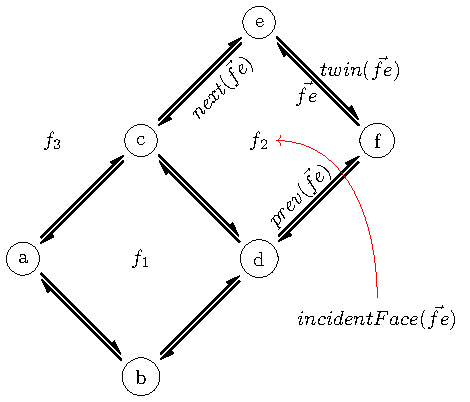
\includegraphics[width=0.6\linewidth]{figures/dcel_example/dcel_example}
    \caption{Components of the DCEL structure.}\label{fig:dcel_example_prime}
\end{figure}

The DCEL data structure has been used in various applications.
For instance, the use of connected edge lists is cardinal to support polygon triangulations and their applications in surveillance (the Art Gallery Problem
\cite{chvatal_combinatorial_1975, orourke_art_1987}) and robot motion planning (Minkowski sums \cite{berg_computational_2008, chew_convex_1993}).
DCELs are also used to perform polygon unions (for example, on printed circuit boards to support the simplification of connected components in an efficient
manner \cite{fogel_cgal_2012}) as well as the computation of silhouettes from polyhedra \cite{fogel_cgal_2012, berberich_arrangements_2010} (applied frequently
in computer vision and 3D graphics modelling \cite{boguslawski_modelling_2011}).

Edge-list data structures have also been utilized for the creation of thematic \textit{overlay maps}. In this problem, the input contains the DCELs of two
polygon layers each capturing geospatial information and attribute data for different phenomena and the output is the DCEL of an overlay structure that combines
the two layers into one.
In many application areas such as ecology, economics and climate change, it is important to be able of join the input layers and match their attributes in order
to unveil patterns or anomalies in data which can be highly impacted by location.
Several operations can then be easily computed given an overlay; for instance, the user may want to find the \textit{intersection} between the input layers,
identify their \textit{difference} (or symmetric difference), or create their \textit{union}.

Spatial databases have been using spatial indexes (R-tree \cite{guttman_r-trees_1984, beckmann_r-tree_1990}) to store and query polygons. Such methods use the \textit{filter and refine}
approach where a complex polygon is abstracted by its Minimum Bounding Rectangle (MBR) that is inserted in the R-tree index.
Finding the intersection between two polygon layers each indexed by a separate R-tree is then reduced to finding the pairs of MBRs from the two indexes that
intersect (filter part).
This is followed by the refine part, which, given two MBRs that intersect needs to compute the actual intersections between all the polygons these two MBRs
contain.
While MBR intersection is simple, computing the intersection between a pair of complex real-life polygons is a rather expensive operation (a typical 2020 US
census track is a polygon with hundreds of edges).
Moreover, using DCELs for overlay operations offers the additional advantage that the result is also a DCEL which can then be directly used for subsequent
operations.
For example, one may want to create an overlay between the intersection of two layers with another layer and so on.

Even though the DCEL has important advantages for implementing overlay operations, current approaches are sequential in nature.
This is problematic considering layers with thousands of polygons. For example, the layer representing the 2020 US census tracks contains around 72K polygons;
the execution for computing the overlay over such large file crashed on a stock laptop. To the best of our knowledge there is no scalable solution to compute
overlays over DCEL layers.

In this paper we describe the design and implementation of a \textit{scalable} and \textit{distributed} approach to compute the overlay between two DCEL layers.
We first present a partition strategy that guarantees that each partition collects the required data from each layer DCEL to work independently, thus minimizing
duplication and transmission costs over 2D polygons.
In addition, we present a merging procedure that collects all partition results and consolidates them in the final combined DCEL.
Our approach has been implemented in a parallel framework (i.e., Apache Spark).

Implementing a distributed overlay DCEL creates novel problems.
First, there are potential challenges which are not present in the sequential DCEL execution.
For example, the implementation should consider features such as \textit{holes} which could lay on different partitions.
Such features need to be connected with their components residing in other partitions so as to not compromise the correctness of the combined DCEL.
Secondly, once a distributed overlay DCEL has been built, it must support a set of binary overlay operators (namely \textit{union, intersection, difference} and
\textit{symmetric difference}) in a transparent manner.
That is, such operators should take advantage of the scalability of the overlay DCEL and be able to run also in a parallel fashion.
Additionally, users should be able to apply the various operators multiple times without the need of rebuild the overlay DCEL data structure.

%The rest of this paper is organized as follows. Section \ref{sec:related} presents related work while Section \ref{sec:prelim} discusses the basics of DCEL 
%and the sequential algorithm.  In Section \ref{sec:methods} we present a partitioning scheme that enables parallel implementation of the overlay computation 
%among DCEL layers; we also discuss the challenges presented in the DCEL computations by distributing the data and how to solve them efficiently.  Two 
%important optimizations are introduced in Section \ref{sec:alternative_methods}.  An extensive experimental evaluation appears in Section 
% \ref{sec:experiments}.


